% \documentclass{beamer}
\documentclass[handout]{beamer}

\usepackage{amsmath}
\usepackage{datetime2}
\usepackage{natbib}

\DTMnewdatestyle{mydateformat}{%
  \renewcommand{\DTMdisplaydate}[4]{%
    \number##1\ % year
    \DTMenglishmonthname{##2}\ % Month
    \number##3% day
  }%
  \renewcommand{\DTMDisplaydate}{\DTMdisplaydate}%
}
\DTMsetdatestyle{mydateformat}

\bibliographystyle{unsrtnat}

% get rid of junk
\usetheme{default}
\beamertemplatenavigationsymbolsempty
\hypersetup{pdfpagemode=UseNone} % don't show bookmarks on

% named colors
\definecolor{foreground}{HSB}{0,0,200}
\definecolor{background}{HSB}{0,0,30}
\definecolor{title}{HSB}{0,0,230}
\definecolor{subtitle}{HSB}{0,0,180}
\definecolor{gray}{RGB}{155,155,155}

% use those colors
\setbeamercolor{titlelike}{fg=title}
\setbeamercolor{subtitle}{fg=subtitle}
\setbeamercolor{institute}{fg=gray}
\setbeamercolor{normal text}{fg=foreground,bg=background}
\setbeamercolor{item}{fg=foreground} % color of bullets
\setbeamercolor{subitem}{fg=gray}
\setbeamercolor{itemize/enumerate subbody}{fg=gray}

\setbeamertemplate{itemize subitem}{{\textendash}}

\setbeamerfont{itemize/enumerate subbody}{size=\footnotesize}
\setbeamerfont{itemize/enumerate subitem}{size=\footnotesize}
\setbeamerfont{title}{size=\huge}

\setbeamertemplate{title page}{
\begin{center}
    {\usebeamerfont{title}\usebeamercolor[fg]{title}\inserttitle}\\[1ex]
    {\usebeamerfont{subtitle}\usebeamercolor[fg]{subtitle}\insertsubtitle}\\[2em]
    {\usebeamerfont{author}\usebeamercolor[fg]{author}\insertauthor}\\
    {\usebeamerfont{institute}\usebeamercolor[fg]{institute}\insertinstitute}\\[.5ex]
    \insertdate
\end{center}
}

\title{Persistent Homology}
\subtitle{Computations and Applications}
\author{Stephen Ermshar}
\institute{Walla Walla University}
\date{\DTMDisplaydate{2020}{2}{7}{}}


\begin{document}




\begin{frame}
    \titlepage
\end{frame}



\begin{frame}{What is Persistent Homology?}
		\begin{itemize}[<+->]
			\item ``\textbf{Persistent homology} describes the changes in homology when a certain scale parameter is varied.''
			\item ``\textbf{Homology} is a mathematical formalism used to define and identify basic topological features, called holes.''
		\end{itemize}
		\begin{figure}[]
			\centering
			\frame{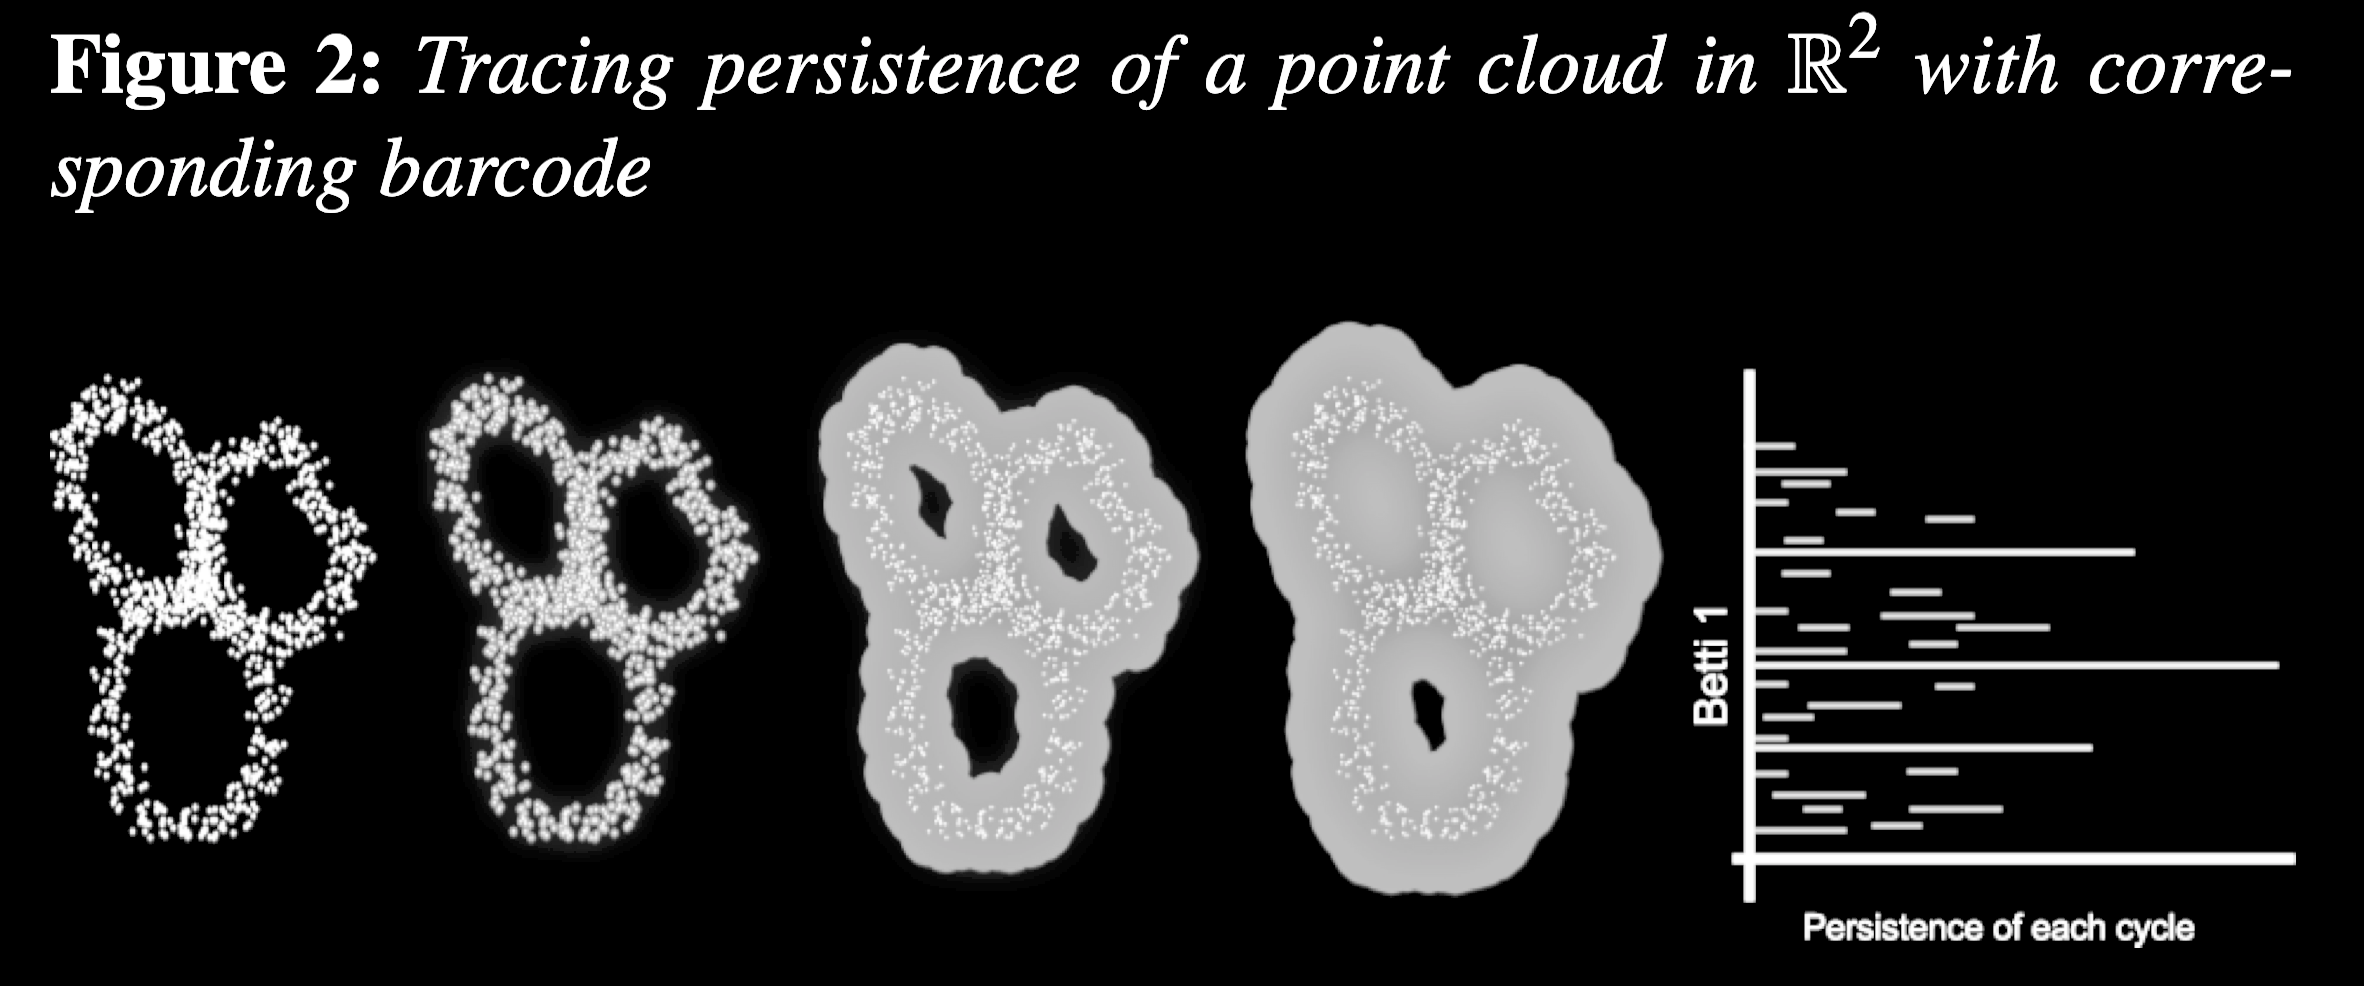
\includegraphics[width=0.8\linewidth]{dey-fig-2.png}}
			\caption{\cite{dey}}
		\end{figure}
\end{frame}



\begin{frame}{References}
	\nocite{wagner}
	\bibliography{../math496-7-zotero.bib}
\end{frame}




\end{document}
